% fig1_magenta_gap.tex: compactification and resolution of the modeled hue circle
% Standalone source for the figure PDF of the same name.
% Build:  pdflatex fig1_magenta_gap.tex
% Drawing taken unchanged from the frozen July manuscript, jmp/Magenta_Gap_JMP.tex, lines 206-261.
% Rebuilt as a standalone vector drawing so that the PDF contains only the figure.
% The border pads the drawing to 410 x 140 pt, the size of the file it replaces,
% so the figure keeps its reviewed scale in the manuscript.
\documentclass[tikz,border={9.33pt 14.65pt}]{standalone}
\usepackage[T1]{fontenc}
\usepackage{lmodern}
\usepackage{amsmath,amssymb}
\usepackage{xcolor}
\usetikzlibrary{arrows.meta,positioning,calc,decorations.pathreplacing}
\begin{document}
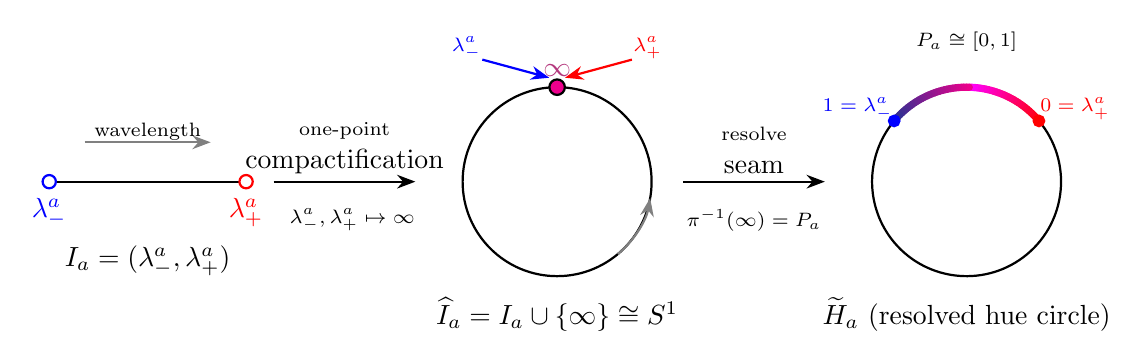
\begin{tikzpicture}[>=Stealth, line width=0.8pt, every node/.style={inner sep=1.5pt}]

  \begin{scope}[shift={(0,0)}]
    \draw (-1.25,0) -- (1.25,0);
    \draw[blue, fill=white] (-1.25,0) circle (2.4pt);
    \draw[red,  fill=white] ( 1.25,0) circle (2.4pt);
    \node[below=4pt, blue] at (-1.25,0) {$\lambda_-^a$};
    \node[below=4pt, red ] at ( 1.25,0) {$\lambda_+^a$};
    \draw[->, gray] (-0.8,0.5) -- (0.8,0.5)
      node[midway, above=-1pt, black] {\scriptsize wavelength};
    \node[anchor=north] at (0,-0.75) {$I_a=(\lambda_-^a,\lambda_+^a)$};
  \end{scope}

  \draw[->] (1.6,0) -- (3.4,0)
    node[midway, above=1pt, align=center] {\scriptsize one-point\\ compactification};
  \node[align=center, anchor=north] at (2.6,-0.28) {\scriptsize $\lambda_-^a,\lambda_+^a \mapsto \infty$};

  \begin{scope}[shift={(5.2,0)}]
    \draw (0,0) circle (1.2);
    \filldraw[draw=black, fill=magenta] (90:1.2) circle (2.8pt);
    \node[above=2pt, magenta!70!black] at (90:1.2) {$\infty$};
    \node[blue] at (-1.15,1.7) {\scriptsize $\lambda_-^a$};
    \node[red ] at ( 1.15,1.7) {\scriptsize $\lambda_+^a$};
    \draw[->, blue] (-0.95,1.55) -- (-0.1,1.32);
    \draw[->, red ] ( 0.95,1.55) -- ( 0.1,1.32);
    \draw[->, gray] (310:1.2) arc (310:350:1.2);
    \node[anchor=north] at (0,-1.4) {$\widehat{I}_a = I_a \cup \{\infty\} \cong S^1$};
  \end{scope}

  \draw[->] (6.8,0) -- (8.6,0)
    node[midway, above=1pt, align=center] {\scriptsize resolve\\ seam};
  \node[align=center, anchor=north] at (7.7,-0.28) {\scriptsize $\pi^{-1}(\infty)=P_a$};

  \begin{scope}[shift={(10.4,0)}]
    \draw (40:1.2) arc (40:-220:1.2);
    \foreach \k in {0,...,29}{
    \pgfmathsetmacro{\a}{40+50*\k/30}
    \pgfmathsetmacro{\b}{40+50*(\k+1)/30}
    \pgfmathtruncatemacro{\p}{100*(29-\k)/29}
    \draw[red!\p!magenta, line width=2.6pt, line cap=round] (\a:1.2) arc (\a:\b:1.2);
  }
  \foreach \k in {0,...,29}{
    \pgfmathsetmacro{\a}{90+50*\k/30}
    \pgfmathsetmacro{\b}{90+50*(\k+1)/30}
    \pgfmathtruncatemacro{\p}{100*(29-\k)/29}
    \draw[magenta!\p!blue, line width=2.6pt, line cap=round] (\a:1.2) arc (\a:\b:1.2);
  }
    \filldraw[red ] ( 40:1.2) circle (1.9pt);
    \filldraw[blue] (140:1.2) circle (1.9pt);
    \node[above left=-2pt,  blue] at (140:1.2) {\scriptsize $1=\lambda_-^a$};
    \node[above right=-2pt, red ] at ( 40:1.2) {\scriptsize $0=\lambda_+^a$};
    \node at (90:1.78) {\scriptsize $P_a \cong [0,1]$};
    \node[anchor=north] at (0,-1.4) {$\widetilde{H}_a$ (resolved hue circle)};
  \end{scope}

\end{tikzpicture}
\end{document}
